\documentclass[./thesis.tex]{subfiles}


\begin{document}
\label{chap:CIPSI}


\section{The basic algorithm}
My initial and most important work has been the improvement of the CIPSI algorithm present in the \QP, that had been implemented by my predecessor.\cite{giner:tel-01077016} As was briefly described in section~\ref{sec:meth_cipsi}, it is an \emph{on the fly} iterative selection algorithm, where determinants are added to the variational wavefunction according to a perturbative criterion. Because it gathers a large amount of information, this CIPSI algorithm has been the basis for other subsequent works presented in the next chapters.

The $n^\text{th}$ iteration of CIPSI can be described like so:

\begin{enumerate}
\item

The variational function $\ket {\Psi^{(n)}}$ is defined over a set of determinants $  \mathcal{D}^{(n)}$ in which we diagonalize $\widehat{H}$
\begin{equation}
\ket{\Psi^{(n)}} = \sum_{I \in \mathcal{D}^{(n)}} c_I^{(n)} \ket{I}
\end{equation}
The determinants in $\mathcal{D}^{(n)}$ will be characterized as \emph{internal}.

\item
For all \emph{external} determinants $\kalpha \notin \mathcal{D}^{(n)}$, we compute a perturbative contribution
\begin{equation}
e_\alpha = \frac{\Hij{\Psi^{(n)}}{\alpha}^2}{E^{(n)} - H_{\alpha \alpha}}.
\end{equation}
%$E^{(n)}$ is an energy that depends on the pertubation theory being used. In our case, the Epstein-Nesbet energy is used.
As we use Epstein-Nesbet perturbation theory, $E^{(n)}=\Evar^{(n)}$ is the variational energy of the wavefunction at the current iteration (note that another perturbation theory could be used here).

\item
From $\{ \alpha \}^{(n)}$ the set of all $\kalpha$ considered at the current iteration, we extract $\{ \alpha^\star \}^{(n)}$ the set of $\kalpha$ of largest contributions $e_\alpha$, and add them to the wavefunction
\begin{equation}
\mathcal{D}^{(n+1)} = \mathcal{D}^{(n)} \cup \{ \alpha^\star \}
\end{equation}

\item
The FCI energy $\EFCI$ can be estimated
\begin{equation}
\EFCI \approx \Evar^{(n)} + \EPT^{(n)}
\end{equation}
with $\Evar^{(n)}$ the variational energy of $\ket {\Psi^{(n)}}$ and
\begin{equation}
\EPT^{(n)} = \sum_{\alpha \in \{\alpha \}^{(n)}} e_\alpha
\end{equation}

\item
Go to iteration $n+1$, or exit on some criterion (number of determinants in the wavefunction, low $\EPT^{(n)}$, \dots).

\end{enumerate}



As can be seen, CIPSI involves the creation of an external space and a precise knowledge of how it interacts with the internal space. Algorithmically speaking, we will need to enumerate all connections between all internal and all external determinants.
There are, perhaps schematically, two ways to do this :

\begin{itemize}
\item
``external to internal'', looping over all possible $\kalpha$ and computing $e_\alpha$.
\item
``internal to external'', looping over all internal determinants $\ket I$ and all single or double excitations $\hat T$, creating $\kalpha = \hat T \ket I$, then incrementing $\tilde e_{\alpha \notin \mathcal{D}}$ by $\Hij{I}{\alpha}$. Finally get $e_{\alpha} = \frac{\tilde e_\alpha^2}{E^{(n)} - H_{\alpha \alpha}}$.
\end{itemize}

%\begin{figure}[h!]
	\begin{center}
		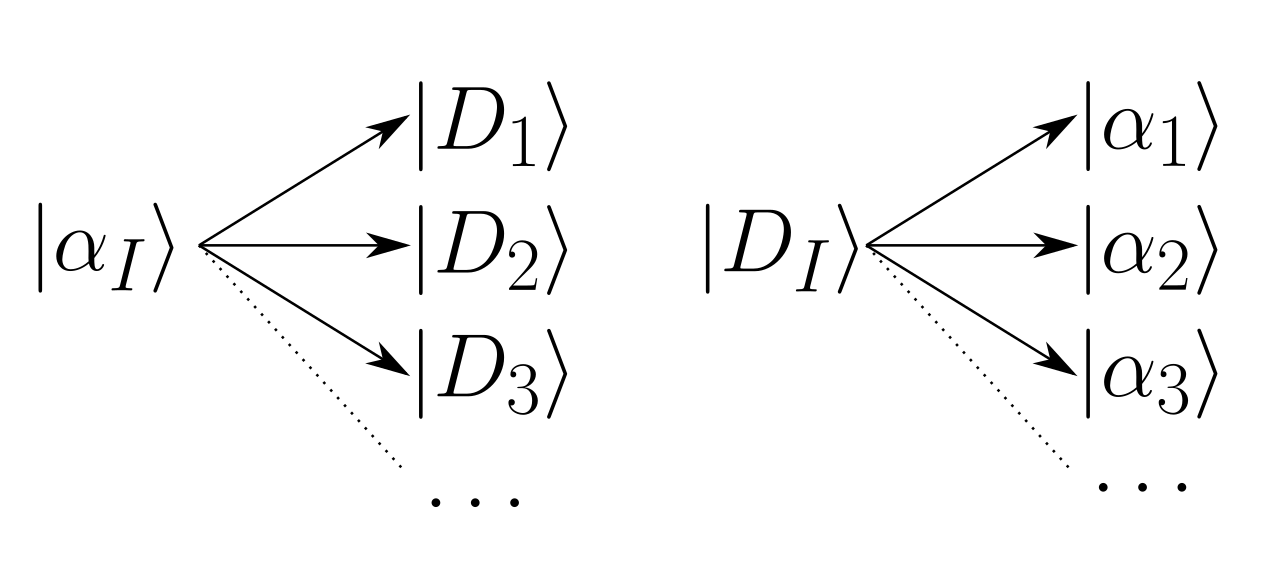
\includegraphics[width=0.4\columnwidth]{figures/matrix_dressing/interactions}
	\end{center}
	%\caption{\label{interactions}}
%\end{figure}

The first approach is less tempting, as it means finding connections between the arbitrary set of internal determinants, and another arbitrary set of $\kalpha$ typically orders of magnitude larger.

While the second approach sounds more straightforward, it has the obvious issue of requiring all $e_\alpha$ to be stored in memory simultaneously. Unfortunately this is usually not feasible, since their number scales as $\order{\Ndet \times \Nalpha^2 \times \qty(\Norb - \Nalpha)^2}$.
The first approach therefore seems simpler when it comes to computing $e_\alpha$, but it begs the question of how to generate all possible $\kalpha$ not simultaneously and with no duplicates. 


\section{Approximations}

Given the qualitative nature of this procedure ---~each $\kalpha$ is either selected or not~--- it is possible to save a vast amount of computation with minimal approximations. These were present in the original implementation and retained in the new one.

Both the former and newer version of CIPSI generate the external space in an ``internal to external'' way, that is, by applying single and double excitations to internal determinants ; a determinant used for creation of $\kalpha$ is referred to as a \emph{generator}.

Ensuring each $\epsilon(\alpha)$ is considered only once, is done by checking all newly generated $\kalpha$ for connection (at most double excitation) to a determinant $\ket {I}$ previously used as a generator ; if a connection $\hat T$ is found, it means $\kalpha$ was already generated from $\ket {I}$ as $\ordering \hat T \ket {I}$.

$D$ is the list of determinants $\kI \in \mathcal{D}$ sorted by decreasing absolute values of $c_I$. Two approximations are made :

\begin{itemize}
\item
The first approximation restricts the set $\{\kalpha\}$. It is very unlikely $\ket \alpha$ will be selected if it is not connected to any $\ket I$ with a large coefficient. Therefore, it is possible to only consider the determinants of larger coefficient as generators. We choose a number of generators $\Ngen$ and only consider $D_{I \leq \Ngen}$ as generators. In practice we set $\Ngen$ according to a norm threshold $n_g$, picking $\Ngen$ as the highest value fulfilling
\begin{equation}
\sum_{I \leq \Ngen} c_I^2 \leq n_g.
\end{equation}
This approximation is a variant of the \emph{three-class CIPSI},\cite{Evangelisti_1983}
and typically $n_g=0.99$ is used in the calculations.
\item The second approximation reduces the cost of $\epsilon_\alpha$.
We do not need extremely accurate values for $\epsilon(\alpha)$ as small differences are unlikely to substantially change the subset of the largest ones.
So  connections to $\ket {D_I}$ with small coefficients $c_I$ can be neglected
in the expression of $\epsilon_\alpha$.
This approximation is achieved in a similar way by defining a threshold $n_s$
on the norm of the wavefunction, and $N_{sel} \geq \Ngen$ a number of so-called
\emph{selectors}. We approximate 
\begin{equation}
  \Hij{\Psi}{\alpha} \approx \sum_{I \leq N_{sel}} c_I \Hij{I}{\alpha}.
\end{equation}
Typically, we use $n_s = 0.999$.

\end{itemize}

Note that generator determinants are a subset of selector determinants. See figure \ref{fig:generators_selectors}.


\begin{figure}[h!]
        
        \begin{center}
                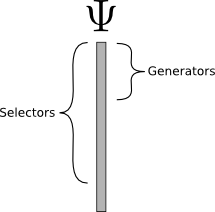
\includegraphics[width=0.25\columnwidth]{figures/cipsi/selexemple2}
        \end{center}
        \caption{$D = \mathcal{D}$ sorted by decreasing ${c_I}^2$ ; generator and selector subsets are defined.}
        \label{fig:generators_selectors}
\end{figure}



\section{Initial implementation}

Originally, the \QP generated the external space in a ``internal to external'' way, by applying all excitations on all determinants ; but the computation of $e_\alpha$ itself was a straightforward ``external to internal'', computing a single $e_\alpha$ at a time, avoiding the problem of keeping track of all $\epsilon(\alpha)$ simultaneously.

\begin{algorithm}
        \caption{Simple CIPSI}
        \label{alg:cipsi_manu}
                \KwData{ $\ket \Psi$ }
                \KwResult{Guarantees all $\epsilon(\alpha)$ are computed only once.}
                $D \gets \mathcal{D}$ sorted by decreasing ${c_I}^2$ \;
                \For {$g \gets 1, \Ngen$}{
                \tcc{apply all double excitations on $|D_g \rangle$}
                \ForAll {$\ket \alpha$ ; $\langle D_g | H | \alpha \rangle \neq 0$}{
                \For{$p \gets 1, g-1$}{
                        \If{$\ket \alpha$ connected to $\ket {D_p}$}{
                                \tcc{$\ket \alpha$ has already been generated by $\ket {D_p}$}
                                discard this $\ket \alpha$ \;
                        }
                }
                \If{$\kalpha \in $ $\{D_{\Nsel+1},\ldots,D_{\Ndet}\}$}{
                        \tcc{$\kalpha \in \mathcal{D}$}
                        discard this $\kalpha$
                }
                 $R \gets 0$ \;
                \For{$s \gets g, \Nsel$}{
                        $R \gets R + c_s \Hij{D_s}{\alpha}$ \;      
                        \tcc{$\ket {D_s}=\kalpha$ is noticed when computing $\Hij{D_s}{\alpha}$}       
                        \If{$\ket {D_s}=\kalpha$}{
                                \tcc{$\kalpha \in \mathcal{D}$}
                                discard this $\ket \alpha$
                        }
                }
                 assert $R = \Hij{\Psi}{\alpha}$  \;
                 $\epsilon(\alpha) = \frac{R^2}{\Evar - \Hij{\alpha}{\alpha}}$
                }
                }
\end{algorithm}

While this relatively simple implementation has been abandoned, it is briefly presented for pedagogical reasons. A slightly more detailed algorithmic version is shown as algorithm \ref{alg:cipsi_manu}.

\begin{enumerate}
\item
$D$ is the list of determinants $\kI \in \mathcal{D}$ sorted with decreasing ${c_I}^2$.
\item
Loop over generators $\ket G$
\item
Generate all singly and doubly excited determinants connected to $\ket G$
\item
From this set, discard those that appear in $\mathcal{D}$. This is now a set of $\ket \alpha$
\item
From this set, discard those that have already been generated before, i.e. those connected to $D_{K<I}$. This is now a set of unique $\ket \alpha$.
\item
Compute $\epsilon(\alpha) = \frac{\langle \alpha|H|\Psi\rangle^2}{\Evar - \Hij{\alpha}{\alpha}}$ for those new $\ket \alpha$.
\end{enumerate}



\section{Principle of the new algorithm}

The current approach is intermediate between computing $\epsilon(\alpha)$ one by one, and keeping track of all of them at the same time.
It creates a subset, or \emph{batch} of external determinants small enough to fit into memory, and importantly, that isn't arbitrary.
A batch is defined by a doubly ionized generator
\begin{equation}
\ket {G_{pq}} = a_p a_q \ket G.
\end{equation}
Determinants contained in the $\ket {G_{pq}}$ batch , some of which may be unique $\kalpha$, can be systematically defined by two indices $r$ and $s$ with
\begin{equation}
\ordering a^\dagger_r a^\dagger_s a_p a_q  \ket G = \Gpqrs.
\end{equation}

Essentially, determinants in a batch are defined by their difference to $\ket{G_{pq}}$. Therefore, comparing $\ket{G_{pq}}$ to a selector determinant allows to systematically determine which $\kalpha$ of the batch it will connect to, and by what excitation. Additional filtering mechanisms are set up to avoid considering selectors that do not interact with the current batch. Those will be made explicit later on. Comparing figures \ref{fig:old_cipsi} and \ref{fig:new_cipsi} hints the differences between the former an newer algorithm. Note that because generators are a subset of selectors, a particular $\kalpha$ generated from $D_g$ must be checked for connection to all selectors either as generators or as selectors.

\begin{itemize}
\item
$D_{1 \le I < g}$ as generators to check if $\kalpha$ has been previously generated
\item
$D_{g \le I \le \Nsel}$ as selectors to compute $\Hij{\Psi}{\alpha}$.
\end{itemize}


\begin{figure}[h!]
        \begin{center}
                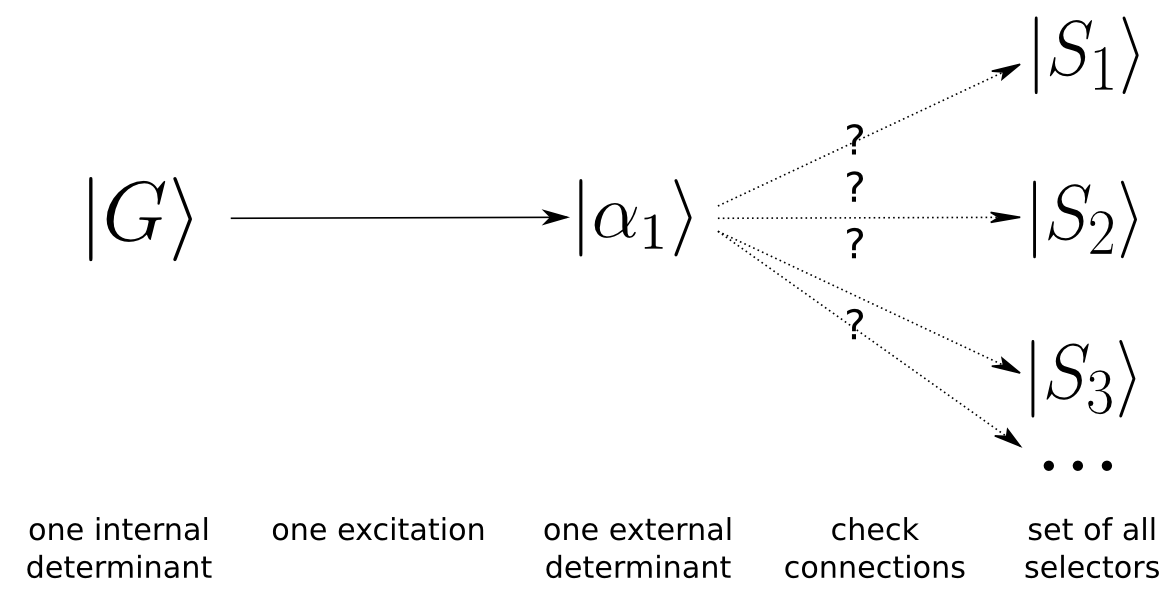
\includegraphics[width=0.6\columnwidth]{figures/cipsi/old_cipsi}
        \end{center}
        \caption{Original CIPSI schematic representation, some details omitted}
        \label{fig:old_cipsi}
\end{figure}


\begin{figure}[h!]
        \begin{center}
                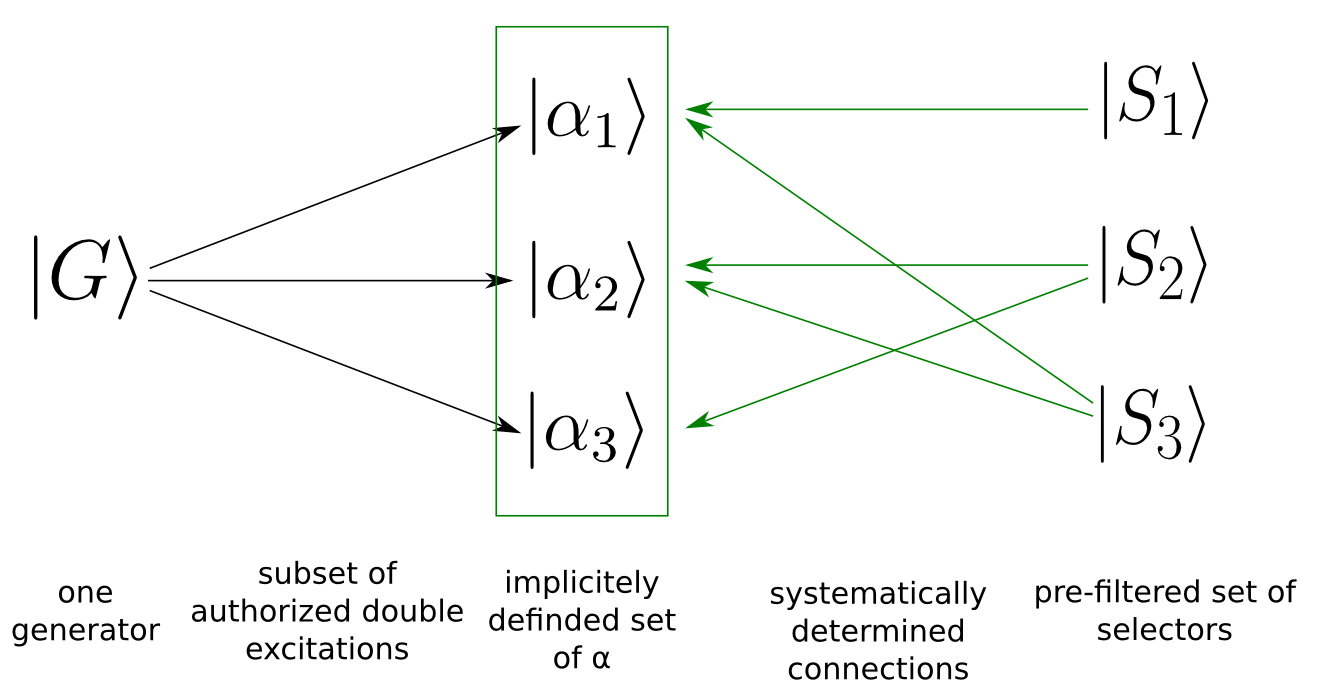
\includegraphics[width=0.6\columnwidth]{figures/cipsi/new_cipsi}
        \end{center}
        \caption{New CIPSI schematic representation, some details omitted.}
        \label{fig:new_cipsi}
\end{figure}

\subsection{Unfiltered algorithm}

Filtering of selectors is a somewhat natural idea that was actually implemented before the batch approach. It however can easily be understood as something added ``on top'' of it, so it will be detailed in the next section and ignored in this one.



\begin{enumerate}
%\setlength{\itemindent}{2em}
\item
Iterate over $\ket {G} \in \left \{ D_{I \leq \Ngen} \right \}$
\item
Iterate over all possible $a_p a_q \ket G = \ket {G_{pq}}$
\item
Allocate a zero-initialized array $P(G_{pq})$ indexed by $r$ and $s$. Each cell is associated with $\ordering a^\dagger_r a^\dagger_s a_p a_q  \ket G = \Gpqrs$. Some cells will be tagged as not being associated with a unique $\ket \alpha$, but either one of :
\begin{itemize}
\item
a determinant already present in the wavefunction
\item
an \emph{exclusion principle violating} determinant (EPV), i.e. $\Gpqrs = 0$
\item
a non-unique $\ket \alpha$ (either a double excitation of a previous generator, or a single excitation of the current one)
\end{itemize}

\item
Since two electrons cannot occupy the same spinorbital, tag cells where $r$ or $s$ is occupied in $\ket {G_{pq}}$ as well as those with $r=s$.
\item
Apply single excitation tagging. This ensures single excitations of $\ket G$ are generated exactly once. It is described in section \ref{single_tagging}.
\item
\textbf{selector loop}: Iterate over $\ket {S} \in \left \{ D_{J \le \Nsel} \right \}$
\item
Determine whether there is a pair $(r,s)$ so that $\ket S = \ket {G_{pq}^{rs}}$. In other words, look for $\ket S$ in the current batch. If there is, tag the corresponding cell, $\Gpqrs \in \mathcal{D}$.
\item
Determine $(r,s)$ pairs so that $\ket {G_{pq}^{rs}}$ is connected to $\ket S$
\item
If $J<I$, tag the corresponding cells ; $\Gpqrs$ has already been generated by $D_J$.
\item
If $J \geq I$, increment all untagged $P_{rs}(G_{pq})$ matrix elements by $\Delta P_{rs}(G_{pq}) = c_J \Hij{S}{G^{rs}_{pq}}$. Note that the excitation operator $\hat{T}$ so that $\ket S=\ordering \hat{T} \Gpqrs$, useful for computing the associated matrix element, can be determined at the same time as the $(r,s)$ pair.
\item
End \textbf{selector loop}. All untagged cells are guaranteed to be associated with a unique $\ket \alpha$ and $P_{rs}(G_{pq}) = \langle \Psi |H|G^{rs}_{pq} \rangle$. $\epsilon(\alpha)$'s for the current batch can be computed  \\

\begin{equation}
\epsilon \qty(\ket {G_{pq}^{rs}}) = \frac{P_{rs}(G_{pq})^2}{\Evar-\Hij{G_{pq}^{rs}}{G_{pq}^{rs}}}
\end{equation}
\item
End of other loops. All $\epsilon(\alpha)$ have been computed a single time.

\end{enumerate}


\subsection{Tagging}

Tagged cells are simply tracked using a boolean matrix $B(G_{pq})$ with $B_{rs}(G_{pq})$ keeping the tag status of $\Gpqrs$, defaulting to $\FALSE$.
In some cases, full columns/rows are to be tagged. Keeping track of fully tagged rows or columns is useful for performance purpose, as it allows to bypass some loop iterations. A simple way to do it, is to add an extra column and an extra row of index $0$ to $B$ ; $B_{0s}(G_{pq}) = \TRUE\,$ means the whole $s$ column is tagged, $B_{r0}(G_{pq}) = \TRUE\,$ means the whole $s$ line is tagged. The actual tag status of $\Gpqrs$ becomes
\begin{equation}
B_{r0}(G_{pq}) \vee B_{0s}(G_{pq}) \vee B_{rs}(G_{pq}).
\end{equation}
While significant, this optimization is fairly simple to set up and use, so for simplification purpose, it will be ignored in the text.


\subsection{Single excitation tagging}
\label{single_tagging}
The algorithm is designed to generate all $\ket {G_{pq}^{rs}}$, which are doubly excited from $\ket G$. The singly excited determinants are not explicitly generated, but are formally present as $\ket{G_{pq}^{ps}}$.
The issue is that $\ket{G_{pq}^{ps}}$ refers to the same determinant $\ordering a^\dagger_s a_q \ket{G}$ regardless of $p$, and the base algorithm only tags a $\kalpha$ as duplicate if it has a previous generator $\ket J$, i.e. if
\begin{equation}
\ket {G_{pq}^{rs}} = \ket {K_{p'q'}^{r's'}} \; ; \; \ket G = D_I \; ; \; \ket J = D_{J<I}
\end{equation}
As can be seen this doesn't cover the case where $G_{pq}^{ps} = G_{p'q}^{p's}$.

To solve this issue, we default to tag $\ket {G_{pq}^{ps}}$, which prevents generating single excitations, and selectively untag in certain cases:


\begin{itemize}
\item
\textbf{Untagging all $\alpha$-spin single excitations of $\ket G$ exactly once}:

Pick $P$ any ``non-frozen'' $\beta$ spinorbital occupied in $\ket G$. We arbitrarily choose the lowest one. Untag $\ket {G_{Pq}^{Ps}}$ whenever $q,s$ are of $\alpha$ spin. Any $\alpha$-spin single excitation $q \rightarrow  s$ is untagged a single time.

$P$ cannot be chosen of $\alpha$ spin, because single excitations $P \rightarrow  s$ and $q \rightarrow  P$ would be formally present as $G_{PP}^{Ps}$ and $G_{Pq}^{PP}$, which aren't ever generated, since for obvious reasons the base algorithm never considers batch $\ket {G_{qq}}$ or determinant $\ket {G_{pq}^{rr}}$.
\item
\textbf{Untagging all $\beta$-spin single excitations of $\ket G$ exactly once}:

Pick $Q$ any ``non-frozen'' $\alpha$ spinorbital occupied in $\ket G$. Again we arbitrarily choose the lowest one. If $p,q$ are of $\beta$ spin, untag $G_{pQ}^{rQ}$. Any $\beta$-spin single excitation $p \rightarrow  r$ is untagged a single time.
\end{itemize}



\section{Systematic determination of connections}

\begin{figure}[h!]
        \begin{center}
                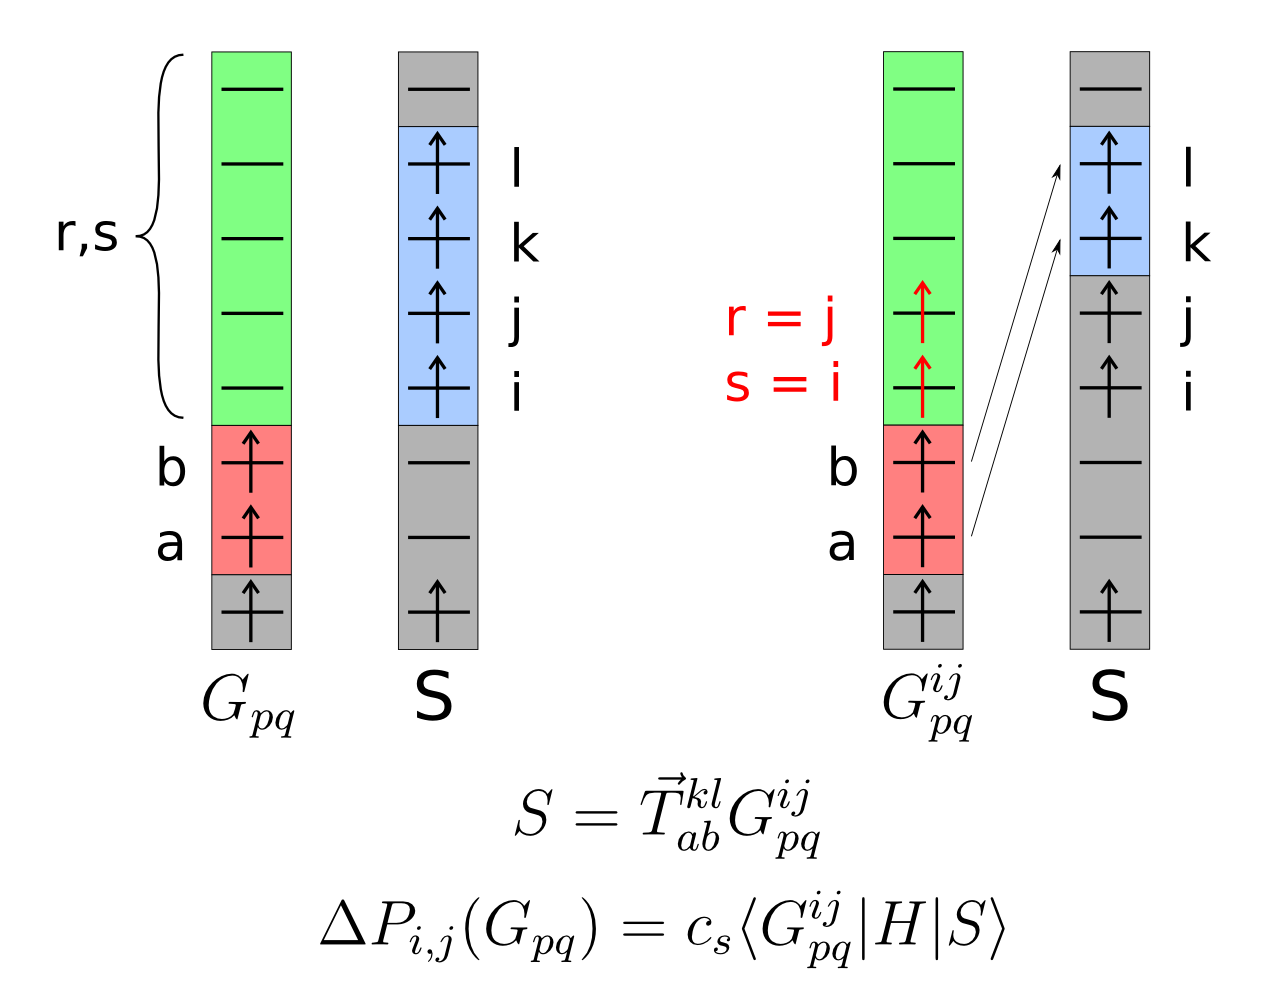
\includegraphics[width=0.70\columnwidth]{figures/cipsi/systematic_determination}
        \end{center}
        \caption{Illustrative example of systematic determination of the connection between a selector $\ket S$ and determinants of the $\ket {G_{pq}}$ batch when $p$ and $q$ have the same spin. \alert{IL FAUT METTRE UN CHAPEAU SUR H DANS LA FIGURE!}}
        \label{fig:systematic_determination}
        
\end{figure}


\begin{figure}[h!]
        \begin{center}
                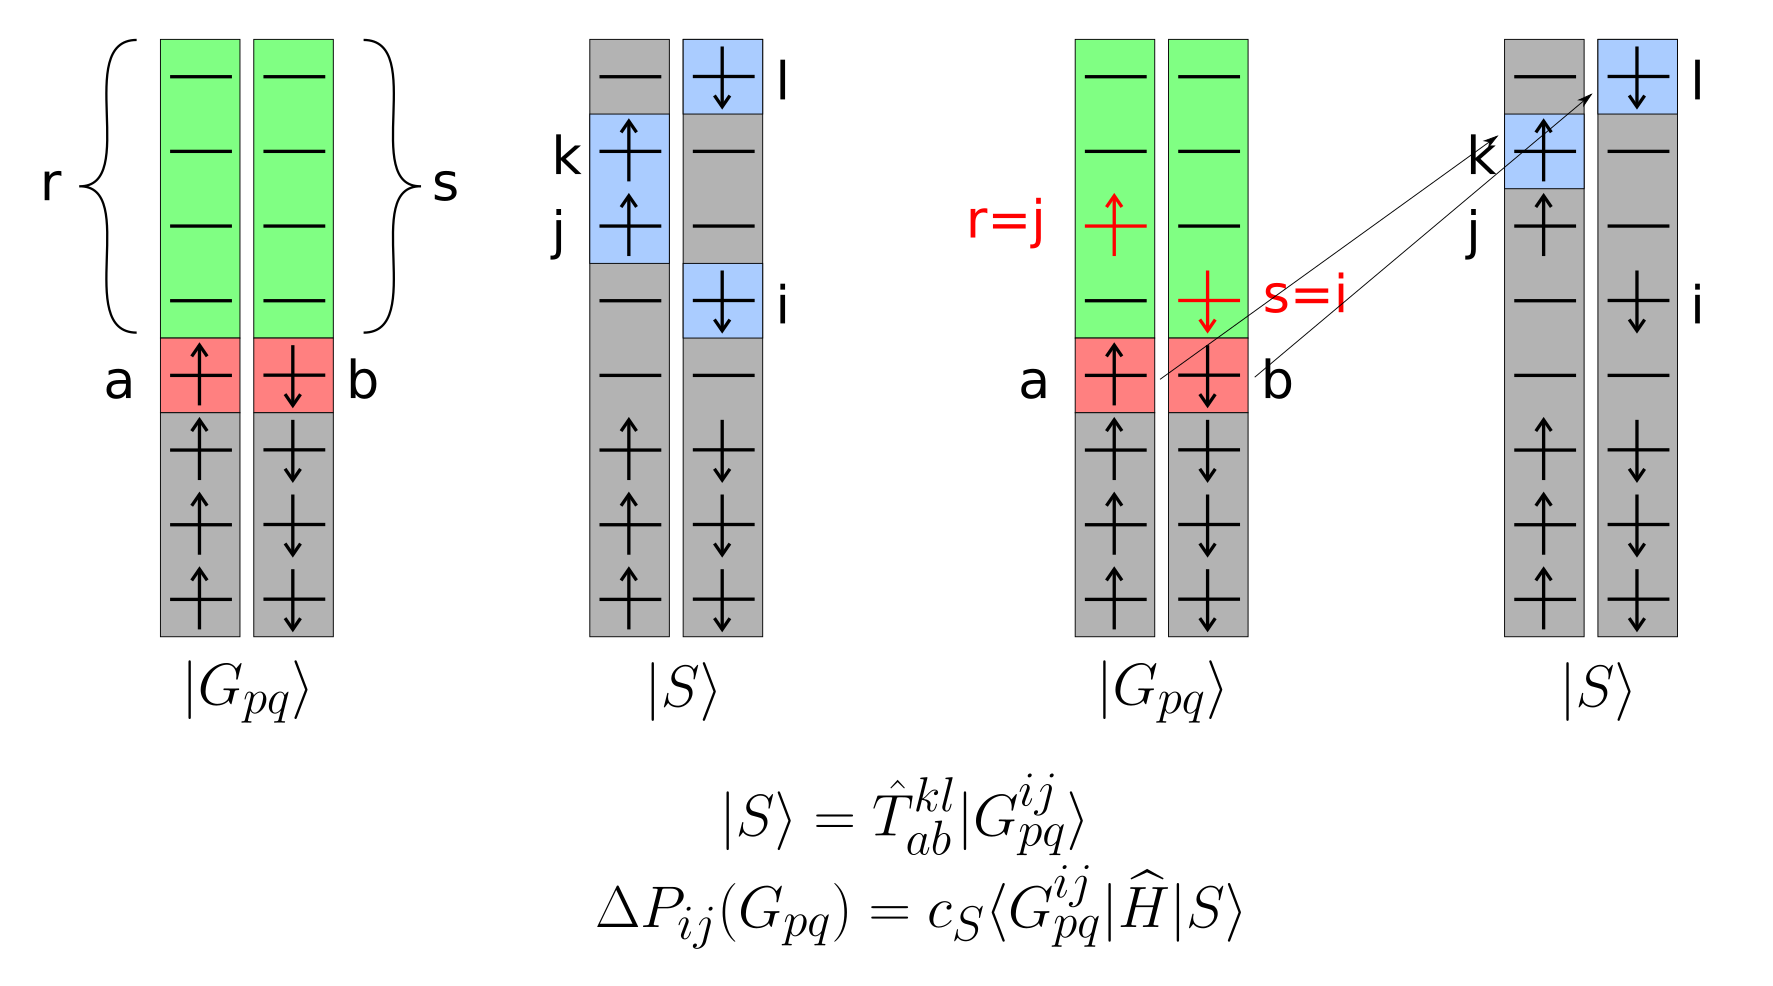
\includegraphics[width=0.90\columnwidth]{figures/cipsi/systematic_determination2}       
        \end{center}
        \caption{Illustrative example of systematic determination of the connection between a selector $\ket S$ and determinants of the $\ket {G_{pq}}$ batch when $p$ and $q$ are of different spins. \alert{IL FAUT METTRE UN CHAPEAU SUR H DANS LA FIGURE!}}
        \label{fig:systematic_determination2}
\end{figure}


The systematic determination of connections between $\ket S$ and determinants from the $\ket {G_{pq}}$ batch is done by comparing $\ket S$ to the doubly ionized determinant $\ket {G_{pq}}$. This yields a set of spinorbitals with different occupation status. Remembering $\ket S$ has two extra electrons compared to $\ket {G_{pq}}$, there are 4 cases of interest:
\begin{itemize}

\item
$i$,$j$ are occupied in $\ket S$ but not in $\ket {G_{pq}}$
\item
$i$,$j$,$k$ are occupied in $\ket S$ but not in $\ket {G_{pq}}$ ; $a$ is occupied in $\ket {G_{pq}}$, but not in $\ket S$
\item
$i$,$j$,$k$,$l$ are occupied in $\ket S$ but not in $\ket {G_{pq}}$ ; $a$,$b$ are occupied in $\ket {G_{pq}}$, but not in $\ket S$
\item
More differences : $\ket S$ isn't connected to any $\ket {G_{pq}^{rs}}$ and can be ignored. 

\end{itemize}

Based on these indices, it is possible to immediately deduce any $(r,s)$ pair so that $\ket {G_{pq}^{rs}}$ is at most a double excitation of $\ket S$, as well as the excitation operator $\hat{T}$ so that $\ket {G_{pq}^{rs}}=\ordering \hat{T} \ket S$. Figures \ref{fig:systematic_determination} and \ref{fig:systematic_determination2} show two possible cases as examples.

While this could be done in a more compact way, we took a ``case by case'' approach, allowing more specialized code for each situation. Taking spin into account, the different cases are listed in table \ref{tab:systematic_determination}.


It is noticeable that, because of the ``wildcard'' indices $X$ and $Y$ :
\begin{itemize}

\item
Cases of the form $a,ijk$ cause full rows/columns of $P(G_{pq})$ to be tagged or incremented.
\item
Cases of the form $ij$ cause the whole $P(G_{pq})$ matrix to be tagged or incremented. Obviously, tagging the whole matrix means stopping the computation for $\ket {G_{pq}}$.
\end{itemize}


\begin{algorithm}
        \caption{Unfiltered CIPSI selection}
        \label{alg:selection}
        \tcc{For simplification purpose, a determinant $\ket S$ is here represented by a single bitstring $S_\sigma$ of size $2\Norb$ where each bit is associated with a spinorbital}
        \KwData{ $\ket \Psi$, i.e. $\{D_I\}$ the set of internal determinants and their coefficients $c_I$}
        \KwData{ $\Ngen$, $\Nsel$, $\Ndet$}
        %\KwResult{ $\Hij{\alpha}{\Psi} \neq 0$ has been computed exactly once for any $\alpha \notin \Psi$ }
        \KwResult{ $e_\alpha \neq 0$ has been computed exactly once for any $\kalpha \notin \{D_I\}$ }
                
        \For{$g \gets 1, \Ngen$}{
        \ForAll{$(p,q) \; ; \; a_p a_q \ket {D_g} \neq 0$}{
                %$\ket {G_{pq}} \gets \ordering a_p a_q \ket {D_g}$\;
                \tcc{$B$ and $P$ are indexed by spinrobitals}
                $B$ a $\FALSE$-initialized boolean matrix of size $2\Norb \times 2\Norb$ \;
                $P$ a zero-initialized real matrix size $2\Norb \times 2\Norb$ \;
                
                apply EPV and single excitations tagging (algorithm \ref{alg:unblock_single}) \;
                
                \For{$t \gets 1,N_{det}$}{
                        $\ket S \gets \ket {D_t}$ \; 
                        $C_\sigma \gets S_\sigma \wedge \neg [G_{pq}]_\sigma$ \; %c \gets \IAND{S}{\NOT{G_{pq}}}$ \; 
                        \If{$||C_\sigma|| = 2$}{
                                $e \gets \texttt{LIST\_FROM\_BITSTRING}(C_\sigma)$\; 
                                $B_{e[1]\, e[2]} \gets \TRUE$\;                     
                        }                       
                        \tcc{see table \ref{tab:systematic_determination} for $(r,s)$ pairs}
                        \uIf{$t < g$}{
                                    
                                \ForAll{$(r, s) \; ; \; \Hij{S}{G_{pq}^{r s}} \neq 0$}{
                                  $B_{rs} \gets \TRUE$ \;
                                } 
                        }
                        \uElseIf{$t \leq \Nsel$}{
                                \ForAll{$(r, s) \; ; \; \neg B_{rs} \wedge \Hij{S}{G_{pq}^{r s}}\neq 0 $ }{
                                  $P_{rs} \gets P_{rs} + c_s \Hij{S}{G_{pq}^{rs}}$ \;
                                }
                        }
                }
                \ForAll{$(r,s) \; ; \; \neg B_{rs}$}{
                  $\kalpha = \Gpqrs$ is a unique $\kalpha$ \;
                  $e_\alpha = \frac{{P_{rs}}^2}{\Evar - \Hij{\alpha}{\alpha}}$ \;
                  %$P_{rs}$ is $\Hij{G_{pq}^{rs}}{\Psi}$ \;
                }
        }
        } 
\end{algorithm}


\begin{algorithm}
        \caption{EPV and single excitations tagging}
        \label{alg:unblock_single}
        \KwData{$B$, $q$, $p$ and $\ket {G_{pq}}$ from outer scope. }
        \KwResult{Updates $B$ so as to tag EPVs, and determinants that were previously generated from a single excitation on $\ket G$}

        \tcc{tag EPV}
                \ForAll{$r \; ; \; (a_r \ket {G_{pq}} \neq 0) \vee (r=p) \vee (r=q)$}{
                        $B_{*r} \gets \TRUE$ \;
                        $B_{r*} \gets \TRUE$ \;
                }
        \tcc{tag duplicate single excitations}
                \If{($q$ is of spin $\alpha$) $\wedge$ ($p$ is the lowest ``non-frozen'' $\beta$ spinorbital)}{
                                $B_{*p} \gets \FALSE$ \;  
                                $B_{p*} \gets \FALSE$ \;          
                        }
                        
                        \If{($p$ is of spin $\beta$) $\wedge$ ($q$ is the lowest ``non-frozen'' $\alpha$ spinorbital)}{
                                $B_{*q} \gets \FALSE$ \; 
                                $B_{q*} \gets \FALSE$ \;         
                        }
\end{algorithm}



\section{Filtering and loop breaking}

A large amount of CPU time is wasted because every doubly ionized generator $\ket {G_{pq}}$ is compared to all internal determinants. In the vast majority of cases, it will show no connection can be made and the internal determinant will be ignored. Thus, it is interesting to filter internal determinants in the outermost loops (loop over generators, and loop over first ionization).

This can be done using the distance $f_A^B = f_B^A$, defined as the minimal number of operations ---~moving, annihilating or creating an electron~--- that must be done to go from a determinant $\ket A$ to a determinant $\pm \ket B$ (i.e. ignoring the phase factor) with respectively $n_a$ and $n_b$ electrons.
Alternatively, it can be defined as the maximum between the number of annihilations and the number of creations required to go from $\ket A$ to $\pm \ket B$.




\begin{equation}
f_A^B = \frac{||A_\alpha \oplus B_\alpha|| + ||A_\beta \oplus B_\beta|| + |n_a-n_b|}{2}
\end{equation}


Considering $\ket S$ a selector determinant and $\ket X$ a generator determinant in a state of ionization from 0 to 2 (it essentially is a wildcard for $\ket G$, $\an p \ket G$ or $\an p \an q \ket G = \ket {G_{pq}}$).

\begin{itemize}
\item
$f_X^\alpha + f_\alpha^S \geq f_X^S$
\item
$\ket \alpha$ can be generated from $\ket X$ iff $f_X^\alpha \leq 2$
\item
$\ket \alpha$ is connected to $\ket S$ iff $f_\alpha^S \leq 2$
\item
$0 \leq (f_Y^S - f_X^S) \leq 1$ with $\ket Y = a_p \ket X$
\end{itemize}


From the rules above, we can deduce that given any $\ket X$ and $\ket S$, there exists an $\kalpha$ generated from $\ket X$ so that $\Hij{\alpha}{S} \neq 0$ only if $f_X^S \leq 4$.
Based on this, a filtering system can be set up, as shown on figure \ref{fig:selection}. The diagram is somewhat convoluted and deserves comments.

\paragraph{Internal determinants' path}
 
A triple loop is shown

\begin{enumerate}
\item
over generators ($G$)
\item
over $p$ a first ionization ($G_p$)
\item
over $q$ a second ionization ($G_{pq}$), i.e. over batches.
\end{enumerate}

In each one some filtering takes place. The determinants of the internal space ``flow'' from the top $\Psi$ into intermediate lists, that are fully constructed before proceeding to the inner loop, as they will be the sources of determinants for that inner loop.
A selector can only be duplicated at the node denoted by a black circle. Otherwise, it follows a single path, always going for the horizontal path if it satisfies the associated condition.
If it doesn't satisfy the condition of a horizontal path, and there is no further vertical path, it is discarded.

\paragraph{``Drop'' instructions}
\emph{Drop} instructions are reached when, predictably, the current loop iteration will not yield any unique $\kalpha$. If a determinant reaches a \emph{drop}, the current loop iteration ends immediately.

\begin{itemize}
\item
\emph{drop} $G_{pq}$ is reached in the case where the whole $P(G_{pq})$ matrix is to be tagged, i.e. the possible values for $(r,s)$ given by table \ref{tab:systematic_determination} are two wildcards ($X,Y$ and $X,\bar Y$).
This corresponds to the case where $\ket {G_{pq}}$ has already been created from a previous generator $\ket K$, i.e. $\ket {G_{pq}} = \ket {K_{p'q'}}$, therefore for any pair $(r,s)$ we have $\ket {K_{p'q'}^{rs}} = \ket {G_{pq}^{rs}}$.\\
\item
\emph{drop} $G_{p}$, in the same fashion, is reached when $\ket {G_{p}}$ has already been created from a previous generator $\ket K$, i.e. $\ket {G_{p}} = \ket{K_{p'}}$. For any triplet $(q,r,s)$ there will be $\ket {K_{p'q}^{rs}} = \ket {G_{pq}^{rs}}$, so no new $\kalpha$ will be created.
\end{itemize}


\paragraph{Paths and loops}
There are roughly a left and a right path. The reason for this, is that we want to reach \emph{drop} instructions as fast as possible. Incidentally, in each loop, the implementation should prioritize operations that may cause a reach to \emph{drop}.

%Not trying to reach \emph{drop} $G_{PQ}$ means we might completely compute the $P$ matrix, only to find that the last selector determinant tags it entierly, for the reson mentioned above.
%Not trying to reach \emph{drop} $G_{P}$ means we might iterate over batches $\Gpqrs$ that are all to be "tagged out" by a single particular selector.

\begin{enumerate}

\item
The first loop discards some internal determinants and separates the others in two disjoint categories.


\begin{itemize}
\item
Right branch : determinants that may contribute to some $P(G_{pq})$ matrix or tag previously generated $\ket \alpha$. In other words, selectors that may connect to some $\ket {G_{pq}^{rs}}$. 

\item
Left branch : Determinants that aren't selectors, but are equal to some $\ket {G_{pq}^{rs}}$. Being non-selectors, those will not be checked for connection to any $\ket {G_{pq}^{rs}}$, but they still must be checked for equality in order to ensure $\ket {G_{pq}^{rs}} \notin \mathcal{D}$
\end{itemize}


This step sets the complexity of the algorithm with respect to $\Ndet$. Naively, $f_G^S$ must be computed for all pairs of internal determinants, setting the complexity to $\mathcal{O}(\Ndet^2)$.
\begin{algorithm}
\caption{Filtering internal determinants for generator $\ket G$}
\label{alg:generators_filtering}
\KwData{$U_\alpha, U_\beta$~: the set of unique $\alpha$ and $\beta$ strings used
to build the $\Ndet$ determinants}
\For{$S_\alpha \in \{U_\alpha \}$}{
$a \gets \texttt{EXC\_DEGREE}(S_\alpha, G_\alpha)$ \;
\If{$a \leq 2$}{
        find $S_\beta \in \{U_\beta\}_{G_\alpha}$ so that $\text{EXC\_DEGREE}(S_\beta, G_\beta) + a \leq 4$  \; 
}
}
\For{$S_\beta \in \{U_\beta \}$}{
$b \gets \text{EXC\_DEGREE}(S_\beta, G_\beta)$ \;
\If{$b \leq 1$}{
        find $S_\alpha \in \{U_\alpha\}_{G_\beta}$ so that $\text{EXC\_DEGREE}(S_\alpha, G_\alpha) + b \leq 4$  \; 
}
}
\end{algorithm}
Our current implementation quickly discards $f_G^S > 4$ by using a method similar to what we used in the Davidson diagonalization, adapted to seek excitation degrees $\leq 4$ rather than $\leq 2$. The key difference is that, for parallelism reasons, the research has to be done individually for each generator~; that is, we are not computing all $f_G^S$ at the same time, but all $f_G^S$ for a given $G$ separately. The procedure is shown as algorithm \ref{alg:generators_filtering}. The complexity is reduced from $\order{\Ndet^2}$ to $\order{\Ndet^{3/2}}$~: each generator has its $\sigma \in \{\alpha, \beta\}$ part compared to all elements of $\{U_\sigma\}$,
the set of unique $\sigma$-spin strings which scales as $\order{\Ndet^{1/2}}$.




Note that the only point of separating those two categories rather than merging them in the same list, is to avoid additional $past$ and $selector$ tests in the second loop.
%If both those lists were merged, a $selector$ condition would need to be added for reaching the right list of the second loop, and $past$ tests would be performed pointlessly on those determinants that would have gone in the left list of the first loop.
This most likely is of little interest, depending on the implementation.
%$past$ and $selector$ should at worst mean fetching an index in an array of indices, and compare it to $I$ or $N_{sel}$ respectively.
But because it is the actual implementation and because it reduces the number of operations, it is still shown.

\item
The second loop discards some internal determinants and separates the other in two categories, this time not disjoint.

\begin{itemize}
\item
Right branch : Determinants that may contribute to some $\Hij{\Psi}{\alpha}$, i.e. selectors that may connect to some $\ket {G_{pq}^{rs}}$
\item
Left branch : Determinants that may cause tagging or reach \emph{drop}, i.e. any determinant that may be equal to some $\ket {G_{pq}^{rs}}$, and previous generators that may connect to some $\ket {G_{pq}^{rs}}$. Those can be found in both lists built in the first loop.
\end{itemize}

As explained above, if there is a previous generator $\ket K$ so that $a_{p'} \ket K = a_p \ket G$, it will result in $P(G_{pq})$ being fully tagged for any $q$, hence a need to reach \emph{drop} $G_p$ to avoid unnecessary computations.
The reach for \emph{drop} $G_p$ can be put on the path between the right list of the first loop and the left list of the second loop.

Indeed, $a_{p'} \ket K = a_p \ket G$ with $\ket K$ a previous generator translates to
\begin{equation}
(f^K_{G_{p}} = 1) \wedge past
\end{equation}
The right list of the first loop contains all internal determinants so that
\begin{equation}
(f^K_G \leq 4) \wedge selector
\end{equation}
However 
\begin{equation}
f^K_{G_{p}} = 1 \implies f^K_G \leq 1 \implies f^K_G \leq 4
\end{equation}
\begin{equation}
past \implies selector
\end{equation}
\begin{equation}
(f^K_{G_{p}} = 1) \wedge past \implies (f^K_G \leq 4) \wedge selector
\end{equation}

Therefore any internal determinant able to reach \emph{drop} $G_P$ will be present in that list. Trivially, from there it will always take the left path because $f^K_{G_{p}} = 1 \implies f^K_{G_{p}} \leq 2$.


\item
Third loop :
\begin{itemize}

\item
Right branch :
Final filtering to keep only selectors that do connect to some $\Gpqrs$
\item
Left branch : $f_{G_{pq}}^S = 2$ implies there exists $(r,s)$ so that $\ket S=\Gpqrs$. If it is the case:
\begin{itemize}
\item
If $past$
\begin{equation}
\ket S=\ket {G_{pq}^{rs}} \implies \ket {S_{rs}} = \ket {G_{pq}}
\end{equation}
As explained above, it leads to $P(G_{pq})$ being fully tagged, and thus \emph{drop} $G_{pq}$ can be reached.
\item
If $\neg past$, $\ket {G_{pq}^{rs}}$ must be tagged for referring to a determinant of the internal space.
\end{itemize}



\end{itemize}

\end{enumerate}



\newcommand{\Gpq}{\ket {G_{pq}}}
\newcommand{\Gpbq}{\ket {G_{p \bar q}}}

\begin{table}

\caption{Systematic ``case by case'' determination of connections between a selector $\ket S$ and determinants of a batch $\Gpq$} 
\label{tab:systematic_determination}
\begin{center}
\begin{minipage}[l]{0.6\textwidth}
        \begin{tabular}{ c|c|c }
                \hline \hline \rule{0pt}{3ex}
                $\ket S$                                                                        &$ r, s$        & $\hat T$ such that $\ordering \hat T \ket S = \Gpqrs$     \\
                \hline \hline \rule{0pt}{3ex}
                $\ac {ij} \Gpq$                                         & $X,Y$         &$ij \rightarrow XY$            \\
                                                                                        & $X,i$         &$j \rightarrow X$              \\
                                                                                        & $i,j$         &$\hat 1$                    \\
                \hline \rule{0pt}{3ex}
                $\an a \ac {ijk} \Gpq$                          &$X,i$          &$aX \rightarrow jk$            \\
                                                                                        &$i,j$          &$a \rightarrow k$              \\
                \hline \rule{0pt}{3ex}
                $\an {\bar a} \ac {\bar i jk} \Gpq$     &$X,j$          &$\bar a k \rightarrow \bar i X$                \\
                                                                                        &$j,k$          &$\bar a \rightarrow \bar i$            \\
                \hline \rule{0pt}{3ex}
                $\an {ab} \ac {ijkl} \Gpq$                      &$i,j$          &$ab \rightarrow kl$            \\
                \hline \rule{0pt}{3ex}
                $\an {a  \bar b} \ac {ijk \bar l} \Gpq$                 &$i,j$          &$a \bar b \rightarrow k \bar l$                \\
                \hline \rule{0pt}{3ex}
                $\an {\bar a \bar b} \ac {i j \bar k \bar l} \Gpq$      &$i,j$          &$\bar a \bar b \rightarrow \bar k \bar l$              \\
                
                \hline \hline \rule{0pt}{3ex}
                $\ket S$                                                                        &$ r, \bar s$   & $\hat T ; \hat T \ket S = \ket {G_{p \bar q}^{r \bar s}}$     \\
                \hline \hline \rule{0pt}{3ex}
                $\ac {i \bar j} \Gpbq$                          & $X, \bar Y$   &$i \bar j \rightarrow X \bar Y$                \\
                                                                                        & $i,\bar X$            &$\bar j \rightarrow \bar X$            \\
                                                                                        & $X,\bar j$    &$i \rightarrow X$              \\
                                                                                        & $i,\bar j$    &$\hat 1$                    \\
                                                                                        
                                                                                        
                \hline \rule{0pt}{3ex}
                $\an a \ac {ij \bar k} \Gpbq$           &$X,\bar k$             &$aX \rightarrow ij$            \\
                                                                                        &$i,\bar k$             &$a \rightarrow j$              \\
                                                                                        &$i,\bar X$             &$a \bar k \rightarrow j \bar X$                \\
                                                                                        
                \hline \rule{0pt}{3ex}
                $\an {ab} \ac {ijk \bar l} \Gpbq$                       &$i,\bar l$             &$ab \rightarrow jk$            \\
                \hline \rule{0pt}{3ex}
                $\an {a  \bar b} \ac {ijk \bar l} \Gpbq$                        &$i,j$          &$a \bar b \rightarrow k \bar l$                \\
                \hline \rule{0pt}{3ex}
                $\an {a  \bar b} \ac {ij \bar k \bar l} \Gpbq$                  &$i,\bar k$             &$a \bar b \rightarrow j \bar l$                \\
        \end{tabular} 
\end{minipage}
\begin{minipage}[r]{0.3\textwidth}
\begin{itemize}
\item
the bar notation $\bar a$ is used to indicate relative spins
%, i.e. $ab$ means $a$ and $b$ are of same spin, $a\bar b$ means they are of different spin.
\item
$\an{ij\ldots}$ is a compact notation for $\an i \an j \ldots$
\item
$X$ and $Y$ are ``wildcard'' indices referring to any spinorbital unoccupied in both $\ket S$ and $\ket {G_{pq}}$ 
\end{itemize}
%- "is in wavefunction" : $\ket {G_{pq}^{rs}} = S$. There is no need to compute $\langle \ket {G_{pq}^{rs}}|H|S \rangle$ since $\ket {G_{pq}^{rs}}$ is necessarily tagged for being present in the wavefunction.
\end{minipage}
\end{center}
\end{table}


\begin{figure}[h!]
        \begin{center}
                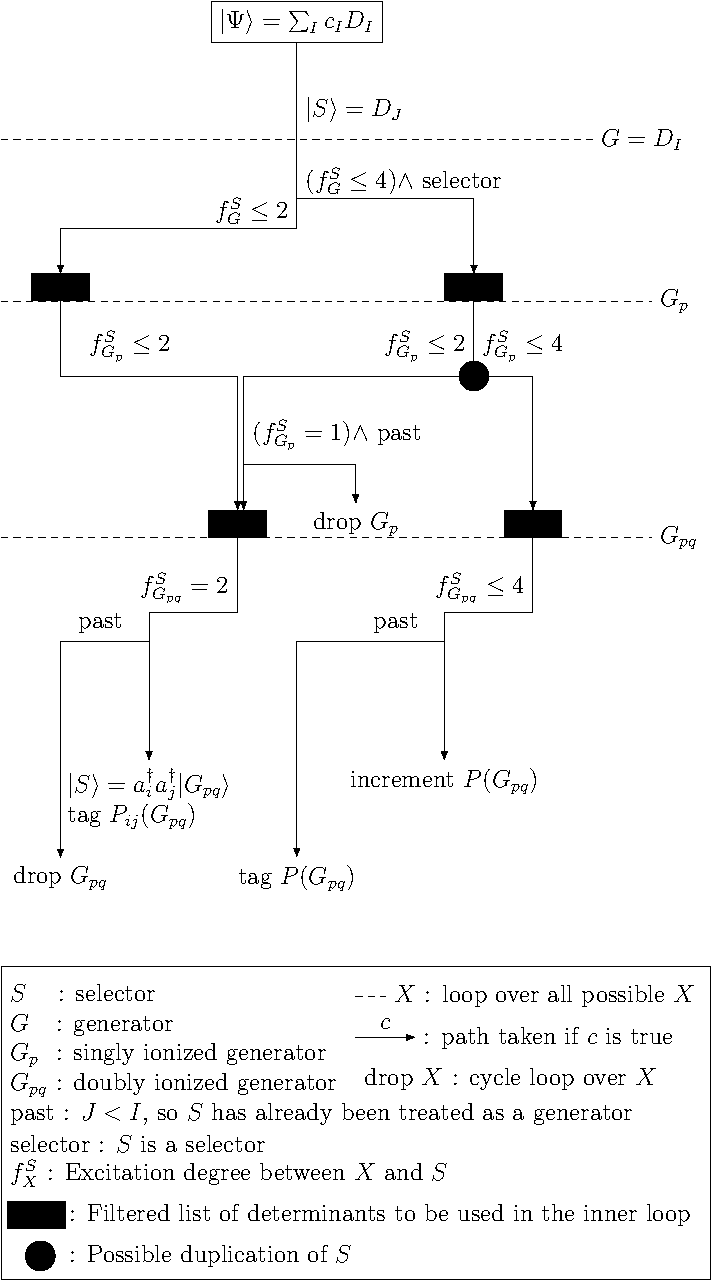
\includegraphics[height=0.90\textheight]{figures/cipsi/selection}
        \end{center}
        \caption{$\ket S$ is the internal determinant currently flowing down the chart.
        Tagging is fully computed, and \emph{drop} instructions eventually reached before any update is done to $P(G_{pq})$.}
        \label{fig:selection}   
\end{figure}

\clearpage
\section{Parallel computation}

Arguably the simplest way to make an algorithm parallel is, whenever possible, to create independent tasks corresponding to one iteration of the outermost loop.
As figure \ref{fig:selection} suggests, iterations for the outermost loop --- over generators --- are independent. This is due to our choice to perform the initial filtering on a ``generator by generator'' basis, giving a total complexity of $\mathcal{O}(\Ndet^{3/2})$ (algorithm \ref{alg:generators_filtering}) ; to achieve $\mathcal{O}(\Ndet)$ the outermost loop would need to be over $\{U_\alpha\}$ and $\{U_\beta\}$. This would give a smaller number of iterations/tasks with extremely unbalanced costs, which does not suit well a parallel scheme. Since in practice the filtering steps only account for a few percent of the total CPU time, we stuck to 1 task = 1 generator. Even so, the cost for different tasks is still very much unbalanced, the first few generators with large coefficients being very expensive, and the cost quickly decreasing.

For a better load balancing, we split the first, expensive tasks into smaller \emph{fragments}, using a fairly simple approach. Essentially, some tasks will require computing just a subset of the $\ket {G_{pq}}$ batches associated with a generator $\ket G$, as opposed to all of them. This implies some overhead, since some filtering steps will be duplicated. Fortunately, only a relatively small number of expensive tasks need to be split.


Each generator $\ket {G_i}$ defines as a ``logical'' task $i$, and for each one we define $F_i$ a fragmentation level, defining the number of independent ``actual'' tasks it should be decomposed in.
We have empirically chosen the following expression for the fragmentation of the tasks:
\begin{align}
F_{\max} & = 1 + \min \qty( \Nelec (\Nelec-1)/2, \lfloor \sqrt{\Nsel} \rfloor/10 ) \\
F_i & = 1 + F_{\max} \qty( \max_{k=1}^{\Nst} |c_{ik}|^{1/2} )
\end{align}
where $F_i$ is an estimated cost of task $i$. In practice $F_i = 1$ for the majority.

Task $i$ is put in the job queue $F_i$ times, each time associated with an index $s$ ranging from $0$ to $F_i-1$, which together with $F_i$ defines the subset of batches this task corresponds to.
%Disjoint subsets are created using modulus, so that subsets are interleaved and thus more balanced.
% Cette phrase n'etait pas facile a comprendre. Le plus simple, c'etait de la virer...
 
\begin{algorithm}
        \caption{Task splitting, pseudocode for master}
        \label{alg:tasksplit_master}
        \tcc{A logical task is the computation of $e[i]$, the sum of $\epsilon(\alpha)$ over all unique $\kalpha$ generated from generator $\ket {G_i}$}
        choose $F_i$ for all $i$\;
        \For{$i=1,\Ngen$}{
        \For{$s=0,F_i-1$}{
                add task $(i,s)$ to the queue   
        }
        }
        $f$,$e$ are arrays size $\Ngen$ initialized with $0$ \;
        \While{not all $e[i]$ printed}{
                get $(i,\text{sum})$ from a slave \;
                $e[i] \gets e[i] + \text{sum}$ \;
                $f[i] \gets f[i] + 1$ \;
                \If{$f[i] = F_i$}{
                        print $e[i]$ \;
                }
        }
\end{algorithm}

\begin{algorithm}
        \caption{Task splitting, pseudocode for slave}
        \label{alg:tasksplit_slave}
        \While{}{
                get task $(i, s \in [0,F_i-1])$ from the queue \;
                $E \gets 0$ \;
                $c \gets 0$ \;
                $G \gets D_I$ \;
                \tcc{duplicated computation if $F_i > 1$}
                filtering for $G$ (see figure \ref{fig:selection}) \;
                \ForEach{$G_p$}{
                \tcc{duplicated computation if $F_i > 1$}
                filtering for $G_p$ (see figure \ref{fig:selection}) \;
                \ForEach{$G_{pq}$}{
                        $c \gets c + 1$ \;
                        \If{$s = c \mod F_i$}{
                                increment $E$ with all unique $\epsilon(\alpha)$ in this batch \;
                        }
                }
                }
                send $(i, E)$ to master \;
        }
\end{algorithm}

This fragmentation scheme is shown in a simpler and more general way when used to compute $\EPT$ in chapter \ref{chap:PT2}. In a nutshell, we can see it as a toy problem where we want to print for each generator the sum of $\epsilon(\alpha)$ over all unique $\kalpha$ it has generated. The algorithm for this on the master and slave side is shown as algorithms \ref{alg:tasksplit_master} and \ref{alg:tasksplit_slave} respectively.


For the determinant selection, we still use the mixed MPI/OpenMP paradigm, where one MPI process per node is used for efficient broadcasting of the replicated data. But, as opposed the Davidson implementation where each task was parallelized with OpenMP, here each OpenMP thread handles independently a task, computed with a single core. The first reason is that the number of tasks is larger than $\Ndet$, which is usually orders of magnitude larger than the number of CPU cores. Moreover, the computation of a task in parallel would require a synchronization barrier at the beginning and the end of the OpenMP section. Here, all the OpenMP threads are completely independent during the whole calculation of the selection, and this explains the very good scaling properties of the implementation, as shown in chapter~\ref{chap:PERF}.

\section{Obtaining spin-pure states}
\label{sec:cipsi_s2}

The presented algorithm generates a wavefunction which is expressed on a truncated space of Slater determinants. Determinants are not necessarily eigenfunctions of the $\widehat S^2$ operator, so the eigenfunctions of the truncated Hamiltonian are not guaranteed to be also eigenfunctions of $\widehat S^2$.

A conventional solution to avoid this issue is to work in the basis of \emph{Configuration State Functions} (CSFs). These are linear combinations of determinants which are eigenfunctions of $\widehat S^2$, and with the desired eigenvalue. Diagonalizing $\widehat H$ in this basis ensures that the solution is spin pure.

Working with CSFs instead of determinants has the additional advantage that the space of CSFs is smaller than the space of determinants. CSFs could in principle be used for CIPSI, but that makes the computation of the matrix elements of $\widehat H$ less straightforward.

We have chosen a more practical solution.\cite{Bytautas_2009} After the selection step, we add to the variational space all the determinants that are necessary to obtain a spin pure solution. These determinants correspond to all the possible spin flips in open shell determinants with the constraint that $\Nalpha$ and $\Nbeta$ are constant. The diagonalization of $\widehat H$ will automatically yield spin pure eigenfunctions at the cost of increasing the size of the wavefunction with many determinants with very small weights.

\section{Conclusion}

The newer CIPSI algorithm runs orders of magnitude faster than the former one thanks to several key improvements.
\begin{itemize}
\item
Excitations do not need to be computed explicitly using algorithms such as those presented in chapter \ref{chap:DET_DRIVEN}. However the associated phase factors still has to be computed.
\item
Although not directly related to the CIPSI algorithm, the computation of the phase factors has been made much cheaper thanks to the use of phase masks (see section~\ref{chap:PHASEMASK})
\item
Selector determinants are simultaneously compared to $(\Norb-\Nalpha)^2$ external determinants $\kalpha$ thanks to the batch system.
\item
Selector determinants go through a filtering mechanism that narrows down the number of selector determinants to be considered against a particular $\kalpha$ (a particular batch of $\kalpha$).
\end{itemize}

This made way for applications that were not affordable before, such as those presented in chapter~\ref{chap:APPLICATIONS}, as well as an additional application to copper complexes.\cite{1806.05115}
The algorithms presented in this chapter also lead to the methods presented in the next chapters.

\end{document}
